\subsection{Test af et moving average filter}
For at teste om moving average filteret overholder de krav der er stillet i \autoref{sec:mavg_krav} visualiseres forskellen mellem det ufiltrede signal og det filtrede signal. Det optagede signal fra pilotforsøget \autoref{sec:pilotforsoeg} sendes til mikrokontrollen via UART-forbindelse, som modtager den retuneret værdi. De sendte og returnerede værdier visualiseres i MATLAB. Resultatet heraf fremgår på \autoref{fig:mavg_test}. 

\begin{figure}[H]
	\centering
	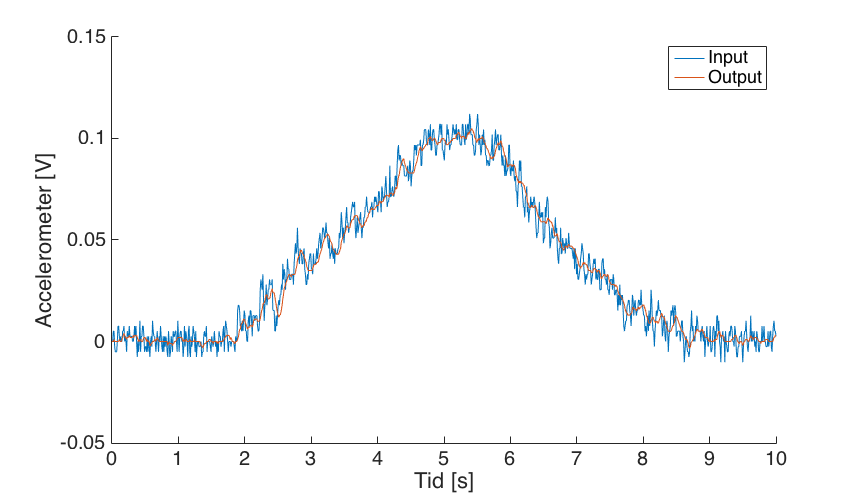
\includegraphics[width=0.5\textwidth]{figures/accelerometer_filter}
	\caption{...}
	\label{fig:mavg_test}
\end{figure}

% Her skal der skrives hvad der kan ses af testen ift ændringerne i signalet. Dernæst vil filteret blive testet ift. det delay der forekommer. 

Da filteret kræver 10 samples for at retunere den første værdi, testes hvorvidt dette stemmer overens med det forventede delay på $100~ms$. Dertil ses også om der forårsages yderligere delay af filteret. Til at måle behandlingstiden, programmeres en timer funktion i mikrokontrolleren, der retunerer behandlingstiden til matlab. Ud fra dette ses et delay på 34 sekunder og 60 milisekunder.

Ud fra ovenstående resultater vurderes det at det filterede signal opfylder kravene for \autoref{sec:mavg_krav}. 